\documentclass{jarticle}
\usepackage{mathtools, multicol}
\usepackage{color}
\usepackage{url}
\usepackage{comment}
\usepackage{here}
\usepackage{txfonts}
\usepackage{listings, jlisting}
\usepackage{latexsym}
\usepackage{subfigure}

\renewcommand{\lstlistingname}{リスト}

\lstdefinestyle{customplain}{
  belowcaptionskip=1\baselineskip,
  breaklines=true,
  frame=tRBl,
  xleftmargin=\parindent,
  language=,
  showstringspaces=false,
  numbers=left,
  basicstyle=\footnotesize\ttfamily,
  keywordstyle=\bfseries\color{black},
  commentstyle=\itshape\color{black},
  identifierstyle=\color{black},
  stringstyle=\color{black},
}

% 余白の設定
\usepackage[top=20truemm, bottom=16truemm, left=10truemm, right=10truemm]{geometry}

% 図の挿入
\usepackage[dvipdfm]{graphicx}

% より複雑な数学記号
\usepackage{amsmath,amssymb}

% 図の通し番号
\usepackage{subfigure}

\newcommand{\todayd}{%
\the\year.{\ifnum \month < 10 0\the\month \else \the\month \fi}.%
{\ifnum \day < 10 0\the\day \else \the\day \fi}}


\makeatletter

\def\@thesis{人工知能}
\def\id#1{\def\@id{#1}}
\def\department#1{\def\@department{#1}}

\def\@maketitle{
	\begin{center}
		{\huge \@thesis \par} %大きなタイトルが記載される部分
		\vspace{10mm}
		{\LARGE\bf \@title \par} % タイトル部分
		\vspace{20mm}
		{\Large 提出締切: 2014.01.02\par} % 提出年月日部分
		\vspace{5mm}
		{\Large 提出日:  \@date \par} % 提出年月日部分
		\vspace{20mm}
		{\Large \@department \par} % 所属部分
		\vspace{10mm}

		{\Large\@id } % 学籍番号部分
		{\Large \@author} % 氏名 
	\end{center}
\par\vskip 1.5em
}

\makeatother

\title{第6回講義課題 課題番号17}
\date{\todayd}
\department{工学部電子情報工学科}
\id{03-123006}
\author{岩成達哉}


\begin{document}

\begin{titlepage}
	\setlength{\topmargin}{1.1in}
	\vspace{100mm}
	\maketitle
\end{titlepage}

\begin{comment}
講義で説明した焼きなまし法の温度を下げるスケジュール において、ギーマンら(S.Geman & D.Geman)の結果 (T(t)≧c/log(1+t)に従って温度を下げていけば 必ず最小値に収束させられること)を分かりやすく説明せよ。単に論文の証明の書き うつしは駄目。高校程度の数学で分かるように平易に説明すること。
ギーマンらの原著論文

Geman and D. Geman. Stochastic relaxation, Gibbs distributions, and the Bayesian restoration of images. IEEE Transactions on Pattern Analysis and Machine Intelligence, 6:721-741, 1984
は ここにある。
また証明の数学的概略は この論文を参照するとよい。
\end{comment}


\section{概要}
本レポートでは,最適化問題を解くためのアルゴリズムの一つである「焼きなまし法」の,温度を下げるスケジューリング方法について説明する.そのために,最適化問題とはなにか,焼きなまし法とはなにかなどを順を追って説明し,最後にギーマンらのスケジューリングの結果について,その方法がなぜよい結果を出せるかを証明を交えながら説明する.

% ----
\section{最適化問題とは}
「ある制約条件のもとで,目的関数を最大あるいは最小にする解を求める」ことを「最適化問題」という.例えば,あなたが家からスーパーに歩いて行くことを想定しよう.家からスーパーに行くまでに様々な経路があるが,あなたは最も時間のかからない道を通りたいと思っている.このときあなたは,いくつかある経路(制約条件)から一つを選び,移動にかかる時間(目的関数)を最小にするという最適化問題を解こうとしているのである.%この場合は,時間$t$という一つの基準のみを対象としているため,その目的関数$f$は$f(x)=t$と一変数の関数として表され,これを最小とするものを経路から選べば良い.

%少し複雑にするために,スーパーまで行くのに自転車やバス,電車などの交通手段を使って良いとすると,目的関数は移動にかかる時間とお金の組み合わせで表されることになるだろう.例えば,自転車で行けば$30$分かかるが,電車で行けば$200$円かかるものの$10$分で到着する場合,時間$t$とお金$c$を天秤にかけて最適な方を選ぶことになる.つまり,この場合の目的関数は$f(t, c)$と二変数の関数として表される.このようにして,多変数の場合も同様に.条件や目的関数を考えることができる.

最適化問題には,目的関数や制約条件によって,いくつかの分類がある.特に,目的関数や制約条件がすべて一次関数(変数が$x_0,\cdots,x_n$,定数が$a_0,\cdots,a_n$のときに,$f=a_0 \cdot x_0 + \cdots + a_n \cdot x_n$のような形の関数)で表されるものを「線形計画問題」,目的関数または制約条件の少なくとも一つが二次以上の関数で表される場合を「非線形計画問題」という.例えば,条件式が$x_1+x_2=2$,目的関数が$f=x_1^2+2 * x^2 \rightarrow min$であるとき,目的関数が一次関数でないので,非線形計画問題に分類される.

% ---
\section{最適化問題の解き方 - 最急降下法 -}
さて,次は最適化問題の解き方の一つである「最急降下法」について説明する.これは,前述の最適化問題のうち非線形計画問題を解く方法の一つで,特に制約条件がない問題に対して有効である.例えば,図\ref{fig:graph}のように,ある関数が与えられた時,その最小値(あるいは最大値)を探す場合に使われる.$x_0$を初期値とし,関数の値を小さくするには$x$軸の正と負どちらに進めばよいかを確認し,小さくなる方に少しづつ進んで,値があまり変化しなくなったところで打ち切るというものである.このように,坂を下っていくイメージとなる.

\begin{figure}[H]
\begin{center}
	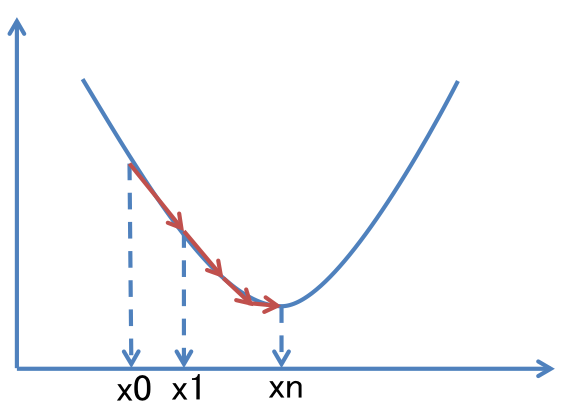
\includegraphics[width=80mm]{image/graph.png}
	\caption{最急降下法の進行}
	\label{fig:graph}
\end{center}
\end{figure}

%さて,値の変化を見る方法は微分

さて,実はこの方法には欠点が存在する.それは,図\ref{fig:two}のように関数に$2$つの谷がある場合,初期値によって,最小値ではない値に収束してしまう場合があることである.一度坂を下って行くと,そこから上には上がらなくなってしまうためであり.このようなとき,求めるべき最適解を「大域的最適解」,局所的に極小となるような解を「局所最適解」と呼ぶ.大域的最適解は局所最適解に含まれる.
\begin{figure}[H]
\begin{center}
	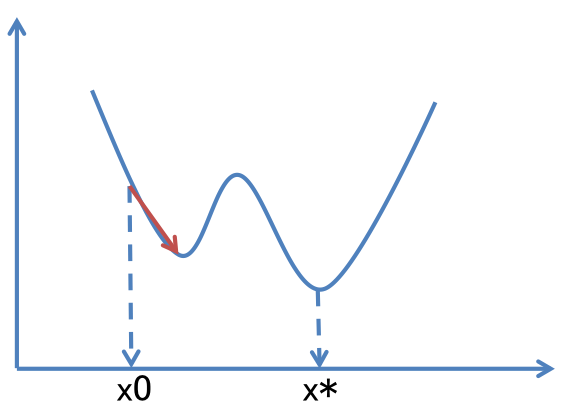
\includegraphics[width=80mm]{image/two.png}
	\caption{最急降下法の欠点}
	\label{fig:two}
\end{center}
\end{figure}


% ---
\section{焼きなまし法とは}
前述のように,最急降下法では,局所最適解に収束してしまう場合があることを示した.これを打開する一つの方法に,「坂を下っていくだけでなく,ある確率で坂を登ることを許す」という手法が考えられる.その手法の一つに「焼きなまし法」がある.

焼きなまし法では,この坂を登るか降りるかを決める確率に「温度」の概念を導入する.温度が高ければ,値の変化量にあまり依存せず,坂を登る確率が高くなるように確率を決め,少しずつこの温度を下げていって,値の変化量に依存するようにして大域的最適解を探すのである.これによって,一度,局所最適解に陥っても,坂を登ることで,大域的最適解にたどりつく確率が上がるのである.

焼きなましとは,金属を加工する際に,徐々に熱を奪っていくことで欠陥を除く手法であり,焼きなまし法はまさにそれになぞらえたアルゴリズムである.また,温度の高いものほど大きなエネルギーを持っているために,谷から出て山を超えられるという物理的なイメージと対応する.


実際の収束の様子をもう少し見てみよう.まず,考えるべきは深さの概念である.図\ref{fig:depth}のように,大域的最適解と局所最適解を分ける山の高さから,それぞれへの深さを$d*$,$d$とする.
%今まで述べたように,焼きなまし法では,局所最適解に陥っても,温度$T$によって.$d$の高さを乗り越えて,大域的最適解に収束する可能性が残ると述べた.
\begin{figure}[H]
\begin{center}
	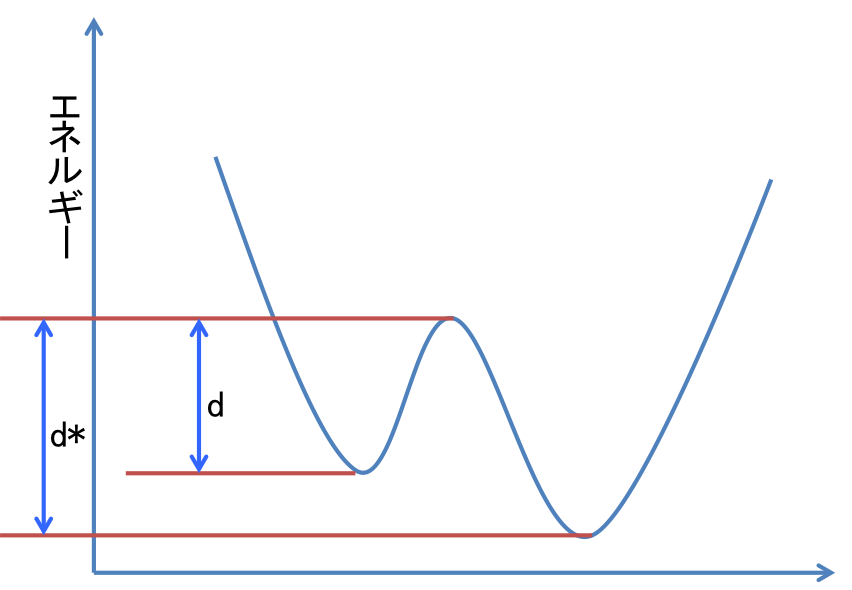
\includegraphics[width=100mm]{image/depth.png}
	\caption{深さの概念}
	\label{fig:depth}
\end{center}
\end{figure}

ここで,ゆっくりと温度を下げていくことを想像してみよう.温度$T$のおかげで,初めは,図\ref{fig:depth}の局所最適解と大域的最適解を自由に行き来できる.少しづつ温度を下げていくと,あるとき$d*$の高さを超えられなくなり,図の右側から左側への遷移がなくなる.しかし,まだ$d$の高さは乗り越えられるため,局所最適解に陥っても図の右側への遷移は可能である.一度右側に移動すると,大域的最適解のところから出られなくなり,結果的に大域的最適解に収束する.

一方で,最終的に局所最適解に収束してしまう場合は,$d*$の高さを超えられなくなってから,まだ局所最適解側の谷にいるうちに$d$の高さを超えられなくなり,局所最適解の谷から出られなくなるときである.つまり,温度を下げることが早過ぎると失敗するのである.

ここでは,温度が下がると,あるときに全く坂を登れなくなるかのように述べたが,実際には坂を登れる確率は$0$にはならない.ただし,その確率があまりにも小さくなるために,超えなくなると見なすことができる.

% ---
%\section{より高度な問題への架け橋}
%さて,ここまで最適化問題を解く方法として,焼きなまし法という手法があることを説明した.これは,温度のパラメータにより,確率的に移動する方向が決まるものであった.この手法は,人工知能の分野にも適用できる.人工知能の分野では,「ニューラルネットワーク」という



% ---
\section{ギーマンらの手法}
%ここまでで,最適化問題を解く方法として,焼きなまし法という手法があることを説明し,焼きなまし法では,温度を徐々に下げて大域的最適解を求めることを説明した.

\subsection{結論}
さて,前述の通り,焼きなまし法で重要なことは,その温度を下げるスケジューリングである.あまりに早く温度を下げすぎれば,結局,大域的最適解にたどりつくまでに坂を登れなくなり,局所最適解に取り残されてしまう.

そこで,ギーマンら(S.Geman \& D.Geman)は以下の様な温度$T$の下げ方をすれば,必ず最小値に収束させられることを示した.
\begin{eqnarray}
	\label{eq:geman}
	T(k) \ge \frac{c}{\log (1+k)}\\
	ただし,kはステップ数,cは定数\nonumber
\end{eqnarray}
さて,この式を見て,「結局$c$が温度の下がる早さを決めてしまうのだから,$c$にも条件が必要だ」と思われたかもしれない.まさにその通りである.結果から言ってしまえば,この$c$の下限は,図\ref{fig:depth}の$d$に相当する.つまり,局所最適解から,大域的最適解へ到達するために必要な高さより大きく$c$を設定しておけばよい.では,なぜこの式が成り立つのかを以降で見ていこうと思う.


\subsection{一般化}
まず,話を少し一般的にするために,あるシステムを考える.このシステムは,様々な状態を取ることができ,状態によってシステムのエネルギー(目的関数)が増減する.例えば,自動販売機では,初めは待機状態にあるが,お金を入れられると購入可能状態になり,商品が買われると,また待機状態に戻る.そして,自動販売機としては,待機状態の方が購入可能状態よりもエネルギーが低いとする.これは,図\ref{fig:auto}のように表せる.前述のスーパーへ買い物に行く例では,経路や交通手段の組み合わせを状態,時間をエネルギーに対応付けられる.

\begin{figure}[H]
\begin{center}
	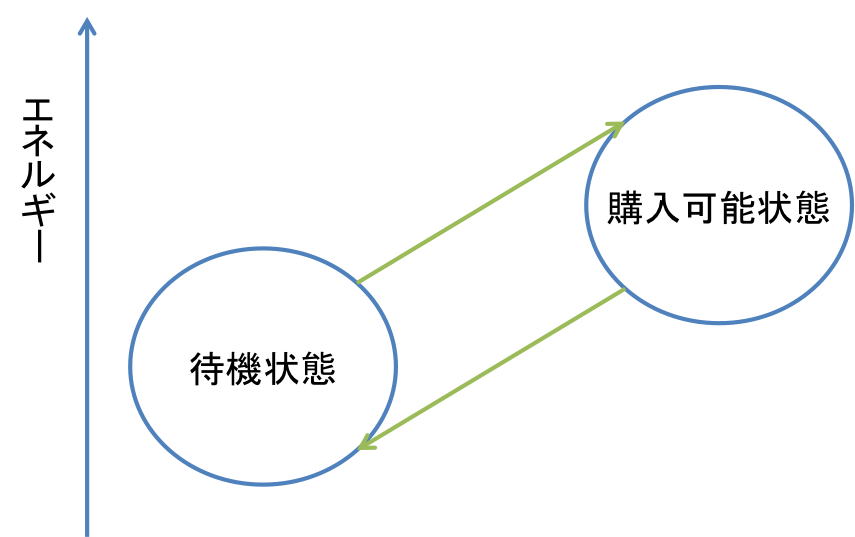
\includegraphics[width=80mm]{image/auto.png}
	\caption{自動販売機の状態変化}
	\label{fig:auto}
\end{center}
\end{figure}

さて,このようなシステムで,エネルギーを最小にするように状態を遷移することを考える.これは,まさに最適化問題の一種であり,単純にエネルギーが小さくなる方に遷移するだけでは,局所最適解へと陥ってしまう.つまり,焼きなまし法を適用することが効果的といえる例である.



\subsection{数式の導入}
\label{sec:intro_eq}

焼きなまし法では,温度$T$と値の変化量を基に次の解の候補を確率的に探すのであった.このシステムでも同様に,遷移先を確率的に選ぶとする.

まず,ある状態$x$から遷移できる状態が$N$個あるときに,そのうちの一つの状態$y$を選ぶ確率は全て同じであるとする関数$R(x, y)$.つまり,
\begin{equation}
	R(x, y) = \frac{1}{N}
\end{equation}
を用意しておく.

次に,それらを選んだ後に,実際にある状態$x$からある状態$y$に遷移できる確率を
\begin{eqnarray}
\label{eq:movable}
&&	p_k =
	\begin{cases}
		1 & (V(y) - V(x) \le 0) \\
		\exp  \frac {-[V(y) - V(x)]}{T_k} & (otherwise)
	\end{cases}\\
	&&ただし,kは遷移した数,V(*)は目的関数(つまりその状態におけるシステムのエネルギー)
\end{eqnarray}
と定める.つまり,次の状態が,エネルギーが低くなる状態でなくても,$0$でない確率で遷移でき,$T_k$が小さくなるに連れて,目的関数が改悪する方向には進みにくくなるのである.これら$2$つの式を用いて,ある状態$s_i$から遷移可能なある状態$s_j$に遷移する確率は
\begin{eqnarray}
	P(s_i, s_j) =
	\begin{cases}
		p_k \cdot R(s_i, s_j) & (i \ne j)\\
		1 - \sum_{h \ne i} p_k \cdot R(s_i, s_h) & (i = j)
	\end{cases}
\end{eqnarray}
とかける.


我々が知りたいのは,このステップを繰り返していったときに,最終的にこのシステムの目的関数$V(x)$を最小にする状態$x$に到達するのかどうかということである.そして,実は式(\ref{eq:geman})が成り立つときに到達するのである.


\subsection{整理}
\ref{sec:intro_eq}節で少し難しい式が出てしまったので,一度整理をしたい.前節で言っていることをまとめると,「ある状態にあるとき,次の移動先として隣合う状態のどれか一つを選ぶ確率は同じであり,実際にその状態に移動する確率はエネルギーが下がる方向なら$1$であるが,上がる方向でも(上がるエネルギー量と温度によるものの)確率は$0$ではない」ということである.もしエネルギーが上がる方向の状態を選び,移動できなかった場合は元の状態にとどまっている.

これを,図\ref{fig:move}を用いて説明すると,$x3$から移動を始めるとすると,隣り合う状態は$x2,x4$の$2$つなので,それぞれを選ぶ確率は$1/2$である.まず,$x2$の方向に移動することを選んだ場合は,$x2$は$x3$に比べてエネルギーが低いため,確実に移動できる.一方で,$x4$は$x3$よりもエネルギーが高いため,$x4$の方向に移動することを選んでも確実に移動するとは限らず,温度とエネルギーの変化量によって,移動する確率が変化する.そして,移動しなかった場合は,$x3$に留まる.
\begin{figure}[H]
\begin{center}
	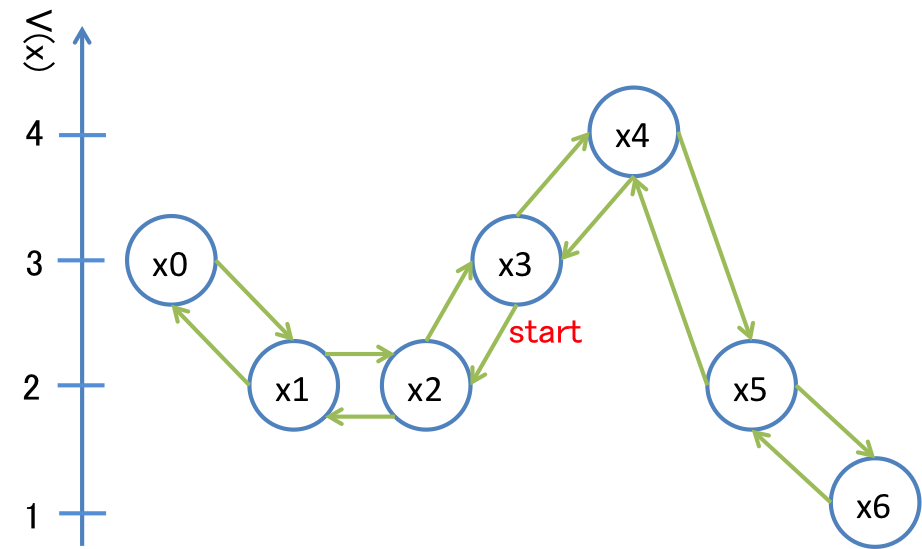
\includegraphics[width=120mm]{image/move.png}
	\caption{移動の例}
	\label{fig:move}
\end{center}
\end{figure}


\subsection{式(\ref{eq:geman})が成り立つ理由}
さて,式(\ref{eq:geman})についてもう一度考えてみよう.我々が知りたいのは,この温度の下げ方で大域的最適解に確実に収束するかということである.見方を変えて考えると,「大域的最適解ではなく,局所最適解に収束する確率が$0$になるか」と言い換えることができる.

極論を言えば,図\ref{fig:depth}のようなときに,$d*$の高さが超えられなくなってから,いつまでたっても$d$の高さは超えられるならば,局所最適解に陥ることはなくなる.つまり,とてもゆっくりと温度を下げていって,これと同等のことが言えるならば,最小値に収束できるということである.

ここで,$d$の高さを超えることのできる確率は,式(\ref{eq:movable})より,
\begin{equation}
\label{eq:pos}
	p_k = \exp \frac{-d}{T_k}
\end{equation}
である.この確率が十分ゆっくりと下がっていけば,局所最適解に陥る確率が$0$となる.その「十分ゆっくり」の基準は,長い目で見てもこの確率がなかなか$0$にならなければよく,ステップを重ねるごとに足した確率の和がいつまでたっても大きくなると考える事ができる.これを式で表すと,いつまでも和を取ると無限に近づいていくということで,
\begin{equation}
\label{eq:inf}
	\sum_{ kをいつまでも大きくしていく} \exp \frac{-d}{T_k} はいつまでも大きくなる
\end{equation}
のようにかけるとしよう.さて,式(\ref{eq:pos})は,$T_k$によってその確率の下がり具合が制御できるが,実は式(\ref{eq:inf})のようになるための,もっとも小さい$T_k$の作り方が式(\ref{eq:geman})なのである.

式(\ref{eq:pos})に,式(\ref{eq:geman})を代入すると,
\begin{equation}
	p_k = \exp [-\frac{d}{c} \log (1 + k) ] = (\frac{1}{1 + k })^ {d/c}
\end{equation}
となる.ここで,$k$を大きくしていくと,$p_k$はどんどん小さくなっていき,$d$が$c$よりも大きければ,その割合が大きくなる.一方で,$c$が$d$よりも大きければ,その変化の割合は小さくなる.式(\ref{eq:inf})のようになるためには,$\frac{1}{1 + k }$の乗数が$1$より小さくなることが必要で,式(\ref{eq:geman})はこの基準を示した式だったのである.


\subsection{拡張とまとめ}
さて,今までの例では,局所最適解と大域的最適解が一つずつ存在する場合だった.しかし,実際のシステムでは,図\ref{fig:move}のように,同じエネルギーの高さを持つ局所最適解や,大域的最適解が複数存在することがある.そのようなときは,局所最適解から大域的最適解に達するために必要な最も大きい高さを$d$とすればよい.これは,その深さ$d$の位置にある局所最適解に留まる確率が,前節の話と同様に,十分$0$と見なしてよくなるからである.

以上をもって,式(\ref{eq:geman})によって,焼きなまし法で最適解が求まることが説明できた.しかし,実際のシステムでこの方法を用いると,収束が遅くなりすぎるために,
\begin{equation}
	T_{k+1} = \alpha T_{k}
\end{equation}
と$\alpha(\text{代表的な値は}0.8 ... 0.9999 \text{など} )$を使って値が小さくなっていく方法などが用いられる.

%まず,ある状態$x$から,ある状態$y$に遷移する確率を$P(x, y)$とする.そして,ある状態$x$から,



\begin{thebibliography}{n}
\bibitem{ref:opt}
『第3章 最適化のアルゴリズム』,\url{http://mikilab.doshisha.ac.jp/dia/seminar/1999/optim/optim01.pdf}

\bibitem{ref:sa_hatena}
『焼きなまし法』,\url{http://d.hatena.ne.jp/Zellij/20120825/p1}

\bibitem{ref:abstract}
BRUCE HAJEK,『COOLING SCHEDULES FOR OPTIMAL ANNEALING』,\url{http://web.mit.edu/6.435/www/Hajek88.pdf},(May 1988)

\end{thebibliography}

\end{document}













